\documentclass[14pt]{extarticle}

\usepackage[english]{babel}
\usepackage[utf8]{inputenc}
\usepackage{hyperref}
\usepackage{graphicx,eso-pic}
\usepackage{newtxtext}
\usepackage{setspace}
\usepackage{multirow}
\usepackage{array}
\usepackage{lipsum}
\usepackage{titlesec}
\usepackage{multicol}
\usepackage{pdfpages}
\usepackage{indentfirst}
\usepackage[bottom=1.5cm,top=2.5cm,left=2cm,right=2cm]{geometry}

\hypersetup{
    colorlinks=true,
    linkcolor=black,
    filecolor=magenta,
    urlcolor=blue,
    pdftitle={Synopsis},
    pdfpagemode=FullScreen,
    }

\urlstyle{same}

\makeatletter

\setlength{\parskip}{1em}

\newcommand\frontmatter{
    \cleardoublepage
    \pagenumbering{roman}
}

\newcommand\mainmatter{
    \cleardoublepage
    \pagenumbering{arabic}
}

\newcommand\backmatter{
    \if @openright
        \cleardoublepage
    \else
        \clearpage
    \fi
}

\makeatother

\titleformat{\section}[block]{\Large\bfseries\filcenter}{}{1em}{}


\title{}
\author{}
\date{}

\begin{document}

\frontmatter

\newgeometry{bottom=2cm,top=2cm,left=1.5cm,right=1.5cm}
\addcontentsline{toc}{section}{Title}
\vspace{-7em}
\maketitle

\vspace{-7em}

\begin{center}
    \singlespacing
\textbf {A Project Work Synopsis} \\

\vspace{1cm}
\onehalfspacing
\emph {Submitted in partial fulfilment for the award of the degree of} \\

\vspace{1.5cm}
\singlespacing

\textbf{
BACHELOR OF ENGINEERING \\
IN \\
COMPUTER SCIENCE and ENGINEERING - INTERNET of THINGS\\
}

\vspace{2.5em}
\onehalfspacing
\textbf{
Submitted by : \\
\begin{tabular}{ccccc}
    Rishabh Anand & Abhishek Singh & Shefali Yadav \\
    19BCS4525 & 19BCS4508 & 19BCS4524 \\
\end{tabular}
}

\textbf{
Under the Supervision of : \\
Nikhil Aggarwal
}

\vspace{1em}

\includegraphics[scale=0.25]{private/seal.png}

\singlespacing

CHANDIGARH UNIVERSITY, GHARUAN, MOHALI - 140413\\
Punjab

\onehalfspacing
August, 2021

\end{center}
\restoregeometry

\newpage

\newpage
\addcontentsline{toc}{section}{Timeline}

\section*{Timeline}
\begin{center}
    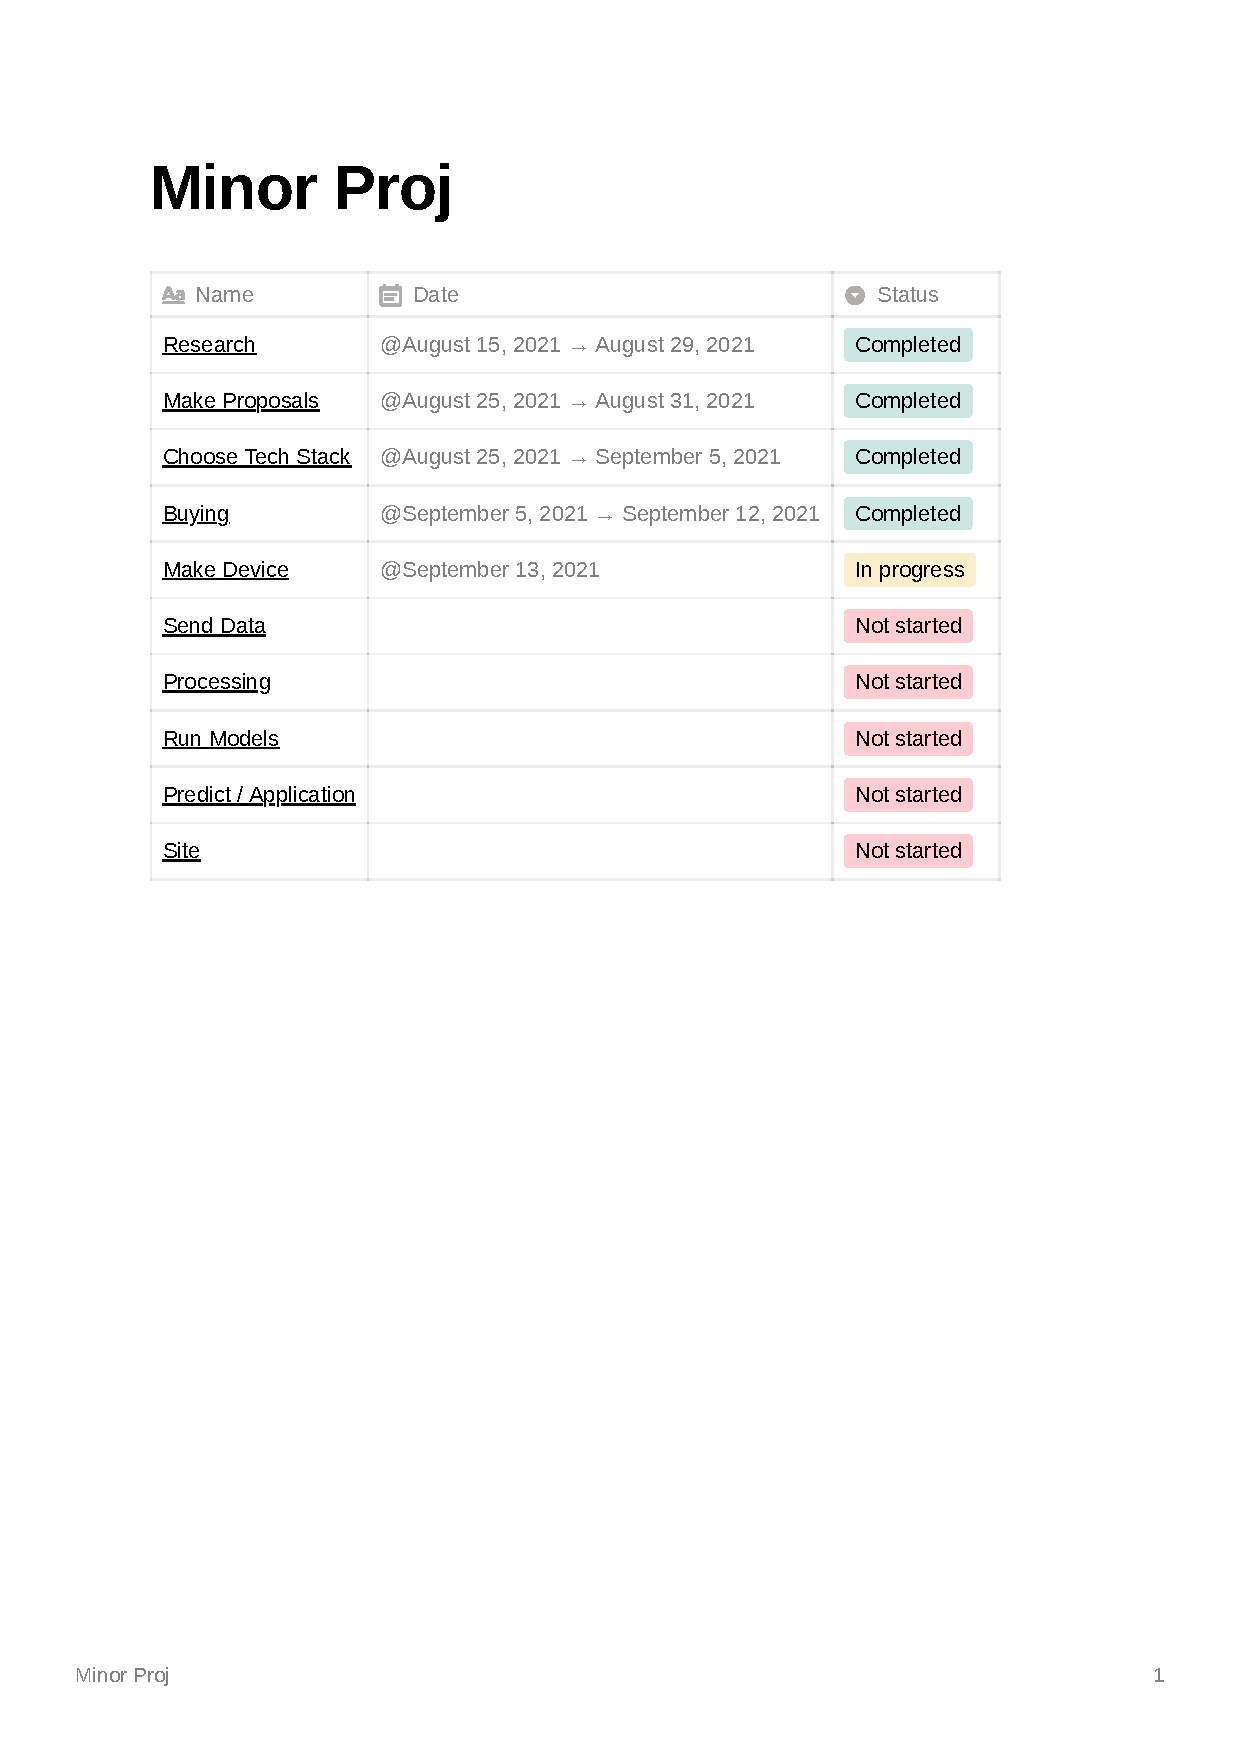
\includegraphics[width=.75\textwidth]{private/gantt.png}
    \includegraphics[width=.75\textwidth]{private/gantt2.png}
\end{center}


\newpage
\addcontentsline{toc}{section}{List of figures}
\listoffigures

\newpage
\addcontentsline{toc}{section}{List of tables}
\listoftables

\setlength{\parskip}{0em}
\newpage
\addcontentsline{toc}{section}{CONTENTS}
\begin{center}
    \tableofcontents
\end{center}

\mainmatter

\setlength{\parskip}{1em}

\newpage
\section{INTRODUCTION}

\par TBD

\par TBD

\subsection{Project Definition}

\par TBD

\begin{itemize}
    \item TBD
\end{itemize}

\newpage
\subsection{Project Overview}

\par TBD

\par TBD

\par TBD

\newpage
\subsection{TBD}
\subsubsection{TBD}
\singlespacing

\par TBD

TBD
\begin{itemize}
    \item TBD
\end{itemize}

% NOTE :: Figures can be added like this.
% \begin{figure}[!h]
%     \centering
%     \includegraphics[width=0.45\textwidth]{private/esp.jpg}
%     \caption{ESP32}
%     \label{fig:esp}
% \end{figure}

\newpage


\newpage
\section{LITERATURE SURVEY}
\subsection{Existing System}

\newpage
\subsection{Proposed System}

\par TBD

\newpage
\subsubsection{Comparision of Various Framworks}

\newpage
\section{PROBLEM FORMULATION}

\par TBD

\newpage
\section{RESEARCH OBJECTIVES}

\par TBD

\newpage
\subsection{The Steps }

\newpage
\subsection{Challanges }

\section{METHODOLOGY}

\backmatter

\newpage
\addcontentsline{toc}{section}{TENTATIVE CHAPTER PLAN}
\section*{TENTATIVE CHAPTER PLAN}

\textbf{CHAPTER 1: INTRODUCTION }

\par This chapter introduces the reader to Federated learning and the basics of the project.

\textbf{CHAPTER 2: LITERATURE SURVEY}

\par This chapter includes the research already available for Applying Federated learning. The findings of the researchers will be highlighted which will become the basis of current implementation. And the existing and current approaches are compared.

\textbf{CHAPTER 3: PROBLEM FORULATION}

\par This chapter covers the basic problem formulations and defines the solution as provided by the paper.

\textbf{CHAPTER 4: RESEARCH OBJECTIVES}

\par This chapter covers the main differences between distributed learning and federated learning. Also, it includes the steps and the challenges of federated learning, how we can use it and how we can overcome the challenges.

\textbf{CHAPTER 5: METHODOLOGY}

\par This chapter covers the technical details of the proposed approach.

\textbf{REFERENCES}

\par This Section contains the references to other documents that are either useful or are directly reffered in this article.


\newpage
\addcontentsline{toc}{section}{REFERENCES}
\section*{REFERENCES}
\begin{enumerate}
    \item TBD
\end{enumerate}

\end{document}